% SOURCE: proposition scope statement (text panel; no plotted data; Prop. 1 first-order identity, A1/A2 named, A4' not required)
% !TEX encoding = UTF-8 Unicode
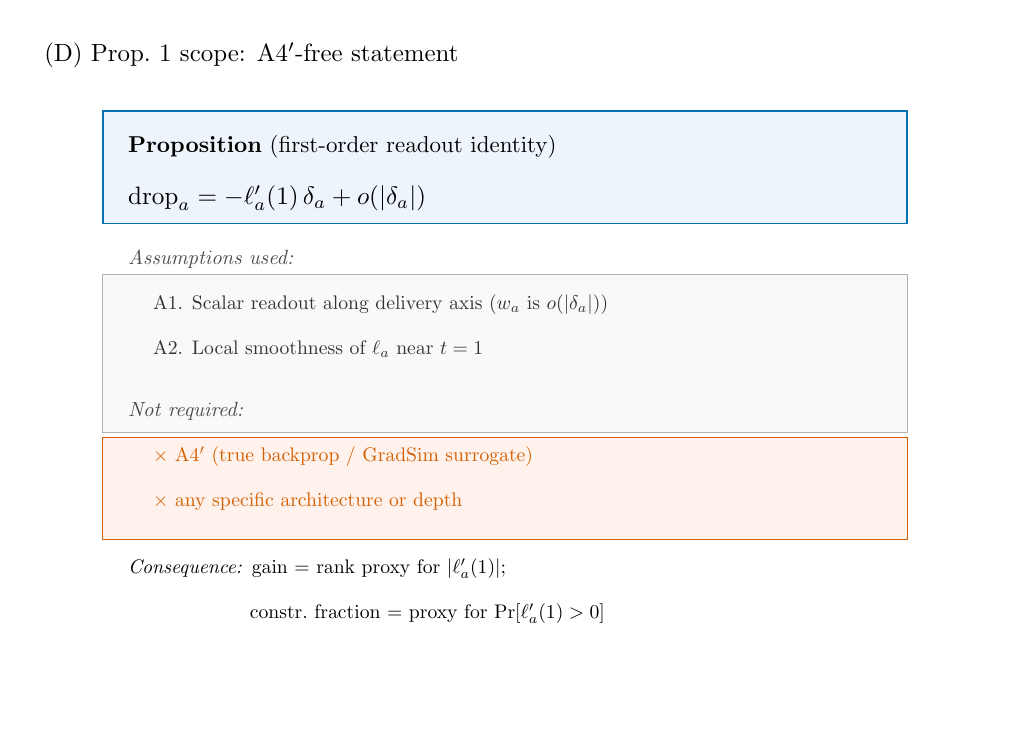
\begin{tikzpicture}[x=1pt,y=1pt]
\definecolor{fillColor}{RGB}{255,255,255}
\path[use as bounding box,fill=fillColor,fill opacity=0.00] (0,0) rectangle (346.90,245.72);
\begin{scope}
\path[clip] (  0.00,  0.00) rectangle (346.90,245.72);

\path[] (  0.00,  0.00) rectangle (346.90,245.72);
\end{scope}
\begin{scope}
\path[clip] (  6.00,  4.00) rectangle (338.90,227.77);
\definecolor{drawColor}{RGB}{0,114,178}
\definecolor{fillColor}{RGB}{238,244,251}

\path[draw=drawColor,line width= 0.5pt,fill=fillColor] ( 27.18,174.88) rectangle (317.71,215.56);
\definecolor{drawColor}{gray}{0.70}
\definecolor{fillColor}{RGB}{249,249,249}

\path[draw=drawColor,line width= 0.3pt,fill=fillColor] ( 27.18, 99.61) rectangle (317.71,156.57);
\definecolor{drawColor}{RGB}{213,94,0}
\definecolor{fillColor}{RGB}{255,242,236}

\path[draw=drawColor,line width= 0.3pt,fill=fillColor] ( 27.18, 60.96) rectangle (317.71, 97.58);
\definecolor{drawColor}{RGB}{0,0,0}

\node[text=drawColor,anchor=base west,inner sep=0pt, outer sep=0pt, scale=  0.83] at ( 36.26,200.52) {\textbf{Proposition} (first-order readout identity)};

\node[text=drawColor,anchor=base west,inner sep=0pt, outer sep=0pt, scale=  0.91] at ( 36.26,181.91) {$\mathrm{drop}_a = -\ell_a'(1)\,\delta_a + o(|\delta_a|)$};
\definecolor{drawColor}{gray}{0.30}

\node[text=drawColor,anchor=base west,inner sep=0pt, outer sep=0pt, scale=  0.74] at ( 36.26,160.13) {\textit{Assumptions used:}};
\definecolor{drawColor}{gray}{0.20}

\node[text=drawColor,anchor=base west,inner sep=0pt, outer sep=0pt, scale=  0.71] at ( 45.34,143.95) {A1. Scalar readout along delivery axis ($w_a$ is $o(|\delta_a|)$)};

\node[text=drawColor,anchor=base west,inner sep=0pt, outer sep=0pt, scale=  0.71] at ( 45.34,127.68) {A2. Local smoothness of $\ell_a$ near $t=1$};
\definecolor{drawColor}{gray}{0.30}

\node[text=drawColor,anchor=base west,inner sep=0pt, outer sep=0pt, scale=  0.74] at ( 36.26,105.20) {\textit{Not required:}};
\definecolor{drawColor}{RGB}{213,94,0}

\node[text=drawColor,anchor=base west,inner sep=0pt, outer sep=0pt, scale=  0.71] at ( 45.34, 89.02) {$\times$ A4$'$ (true backprop / GradSim surrogate)};

\node[text=drawColor,anchor=base west,inner sep=0pt, outer sep=0pt, scale=  0.71] at ( 45.34, 72.75) {$\times$ any specific architecture or depth};
\definecolor{drawColor}{RGB}{0,0,0}

\node[text=drawColor,anchor=base west,inner sep=0pt, outer sep=0pt, scale=  0.71] at ( 36.26, 48.34) {\textit{Consequence:} gain = rank proxy for $|\ell_a'(1)|$;};

\node[text=drawColor,anchor=base west,inner sep=0pt, outer sep=0pt, scale=  0.71] at ( 36.26, 32.06) {\phantom{Consequence:} constr.\ fraction = proxy for $\Pr[\ell_a'(1)>0]$};
\end{scope}
\begin{scope}
\path[clip] (  0.00,  0.00) rectangle (346.90,245.72);
\definecolor{drawColor}{RGB}{0,0,0}

\node[text=drawColor,anchor=base west,inner sep=0pt, outer sep=0pt, scale=  0.90] at (  6.00,233.52) {(D) Prop.\ 1 scope: A4$'$-free statement};
\end{scope}
\end{tikzpicture}
